\begin{figure*}[!t]
\small
  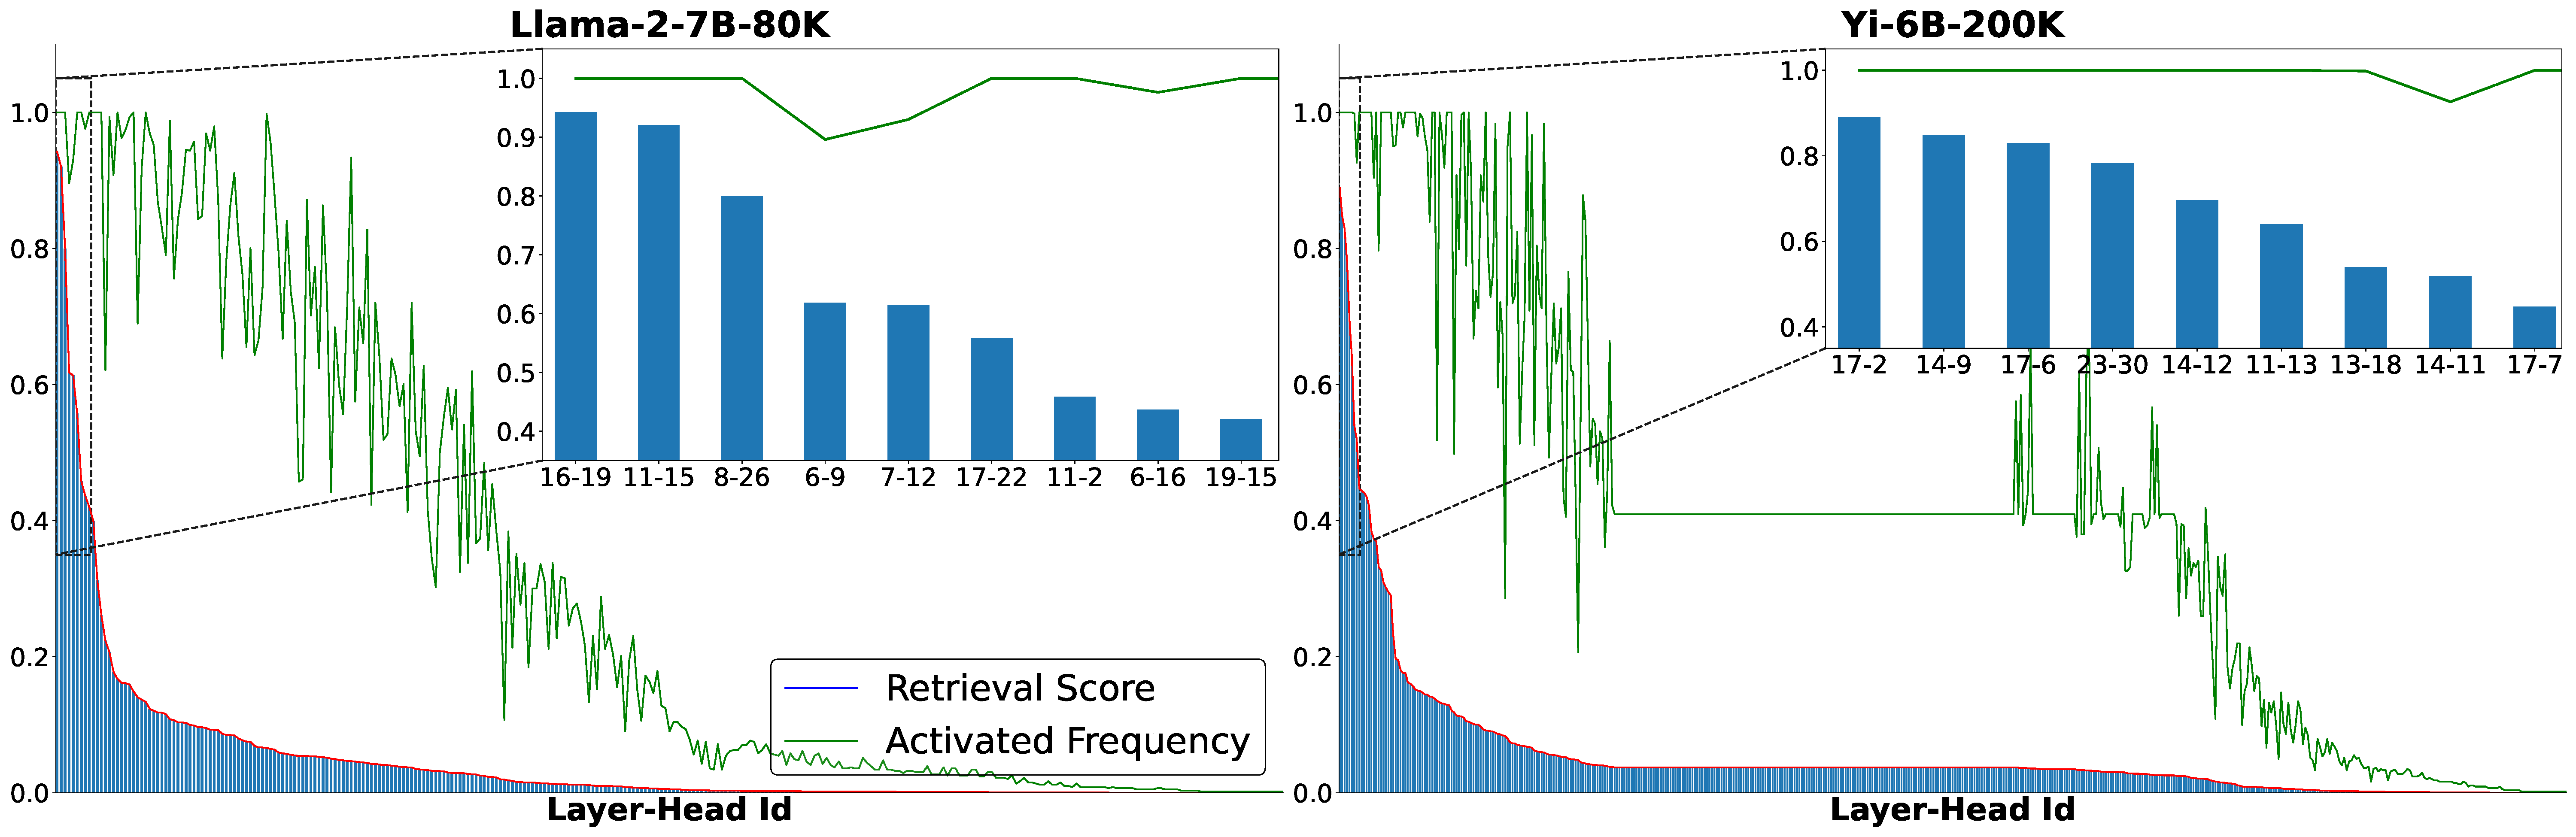
\includegraphics[width=\linewidth]{figures/score_distribution.pdf}
  \caption{Retrieval score (blue): average number of activated tokens; 
  Activation Frequency (green): frequency of at least activated on one token. 
  The \textit{gap} between the two curves shows \textit{context-sensitivity}: a head of high activation frequency but low retrieval score means it is only activated on certain tokens and contexts; a head of high retrieval score means it is activated on almost any context. 
  For both LLaMA and Yi, there exist strong heads that are not sensitive to context and always activated.
  }
  \label{fig:score_dist}
\end{figure*}
